\documentclass[11pt,a4paper]{article}

% --- Paquets standards ---
\usepackage[utf8]{inputenc}
\usepackage[T1]{fontenc}
\usepackage[french]{babel}
\usepackage{amsmath, amsfonts, amssymb, amsthm}
\usepackage{graphicx}
\usepackage{geometry}
\geometry{hmargin=2.5cm,vmargin=2.5cm}
\usepackage{hyperref}
\usepackage{xcolor}
\usepackage{listings}
\usepackage{algorithm}
\usepackage{algpseudocode}
\usepackage{setspace}
\usepackage{caption}
\usepackage{tikz}
\usetikzlibrary{shapes,arrows,positioning,fit,calc,arrows.meta}
\usepackage{booktabs}
\usepackage{enumitem}

\setstretch{1.15}

% --- Configuration du code source ---
\lstset{
    basicstyle=\ttfamily\small,
    keywordstyle=\color{blue}\bfseries,
    stringstyle=\color{red},
    commentstyle=\color{teal},
    frame=single,
    breaklines=true,
    showstringspaces=false,
    captionpos=b
}

% --- Définitions mathématiques ---
\newtheorem{definition}{Définition}
\newtheorem{theorem}{Théorème}
\newtheorem{property}{Propriété}

\title{
    \vfill
    \textbf{\huge Rapport de Projet : Windowing Orthogonal}\\
    \vspace{0.8cm}
    \large \textbf{Structures de Données II (INFO-F-203)}\\
    \vspace{0.4cm}
    \textit{Étude, Conception et Implémentation d'un Index Géométrique en $\mathcal{O}(\log n + k)$}
    \vfill
}
\author{
    \textbf{Réalisé par : Abdellah Boumaiza} \\
    Master 1 en Sciences Informatiques \\
    Faculté des Sciences -- Université de Mons
}
\date{Année Académique 2025-2026}

\begin{document}

\maketitle
\thispagestyle{empty}
\newpage

\tableofcontents
\newpage

% ==============================================================================
\section{Introduction et Problématique}
% ==============================================================================

L'informatique géométrique (\textit{Computational Geometry}) étudie la conception et l'analyse d'algorithmes et de structures de données pour résoudre des problèmes spatiaux complexes. L'un des problèmes fondamentaux de ce domaine est le \textit{windowing} (ou requêtage par fenêtre). Ce problème se pose de manière naturelle dans les Systèmes d'Information Géographique (SIG), la CAO, ou les interfaces graphiques, où il est nécessaire d'afficher uniquement les objets visibles dans la zone d'écran actuelle.

\subsection{Énoncé du problème}

Étant donné un ensemble $S$ de $n$ segments de droites orthogonaux (strictement horizontaux ou verticaux) dans un plan euclidien bidimensionnel $\mathbb{R}^2$, le problème du windowing consiste à identifier tous les segments $s \in S$ qui intersectent une fenêtre de requête rectangulaire $W$, alignée sur les axes.

Face à des jeux de données contenant des millions de segments, une approche naïve — consistant à tester l'intersection de chaque segment avec $W$ — exhiberait une complexité temporelle linéaire $\mathcal{O}(n)$, ce qui est inacceptable pour des applications interactives ou temps réel.

\begin{figure}[h]
\centering
\begin{tikzpicture}[scale=0.8]
    % Axes
    \draw[->] (-4,0) -- (5,0) node[right] {$x$};
    \draw[->] (0,-3) -- (0,4) node[above] {$y$};

    % Fenêtre de requête
    \draw[blue, thick, dashed] (-1,-1.5) rectangle (3,2.5);
    \fill[blue!10, opacity=0.5] (-1,-1.5) rectangle (3,2.5);
    \node[blue] at (1, 0.5) {$W$};

    % Segment horizontal qui intersecte (extrémité dans W)
    \draw[green!60!black, very thick] (-0.5, 1.5) -- (2.5, 1.5)
        node[right, black] {\small horiz. \checkmark};
    \filldraw[green!60!black] (-0.5,1.5) circle (2pt);
    \filldraw[green!60!black] (2.5,1.5) circle (2pt);

    % Segment vertical traversant (aucune extrémité dans W)
    \draw[green!60!black, very thick] (1.5, -2.5) -- (1.5, 3.5)
        node[above, black] {\small vert. \checkmark};

    % Segment horizontal traversant (aucune extrémité dans W)
    \draw[green!60!black, very thick] (-3.5, -0.5) -- (4.5, -0.5)
        node[right, black] {\small traverse \checkmark};

    % Segment en dehors
    \draw[gray, thick] (-3.5, 3) -- (-1.5, 3)
        node[right, black] {\small \textcolor{gray}{hors $W$}};
    \draw[gray, thick] (3.5, -2) -- (3.5, 2)
        node[right, black] {\small \textcolor{gray}{hors $W$}};

    % Labels axes
    \node[below] at (-1,0) {\small $x_{min}$};
    \node[below] at (3,0) {\small $x_{max}$};
    \node[left] at (0,-1.5) {\small $y_{min}$};
    \node[left] at (0,2.5) {\small $y_{max}$};
\end{tikzpicture}
\caption{Illustration du problème du windowing : segments intersectant la fenêtre $W$ (en vert) et segments en dehors (en gris).}
\label{fig:windowing}
\end{figure}

\subsection{Objectif du projet}

L'objectif de ce projet est de concevoir un système d'indexation géométrique capable de répondre à ces requêtes en un temps optimal $\mathcal{O}(\log n + k)$, où $k$ représente la taille de la réponse. Conformément à la théorie développée au Chapitre 10 de l'ouvrage \textit{Computational Geometry} (de Berg et al.), notre solution s'appuie sur une architecture hybride couplant des \textbf{Priority Search Trees} pour la localisation des extrémités et des \textbf{Interval Trees} pour la détection des segments traversants.

% ==============================================================================
\section{Cadre Formel et Notations Mathématiques}
% ==============================================================================

\begin{definition}[Segment Orthogonal]
Un segment de droite $s$ est défini par deux points d'extrémité $p_1 = (x_1, y_1)$ et $p_2 = (x_2, y_2)$. L'ensemble $S$ est composé exclusivement de segments orthogonaux :
\begin{itemize}
    \item $s$ est \textbf{horizontal} si $y_1 = y_2$.
    \item $s$ est \textbf{vertical} si $x_1 = x_2$.
\end{itemize}
\end{definition}

\begin{definition}[Fenêtre de Requête]
Une fenêtre de requête $W$ est un sous-espace rectangulaire fermé de $\mathbb{R}^2$ :
\[ W = [x_{min}, x_{max}] \times [y_{min}, y_{max}] \]
Les bornes peuvent être infinies ($\pm\infty$) pour représenter des fenêtres semi-illimitées.
\end{definition}

\subsection{Condition d'Intersection}

Un segment $s$ intersecte $W$ si et seulement si l'un des trois cas se produit :

\begin{figure}[h]
\centering
\begin{tikzpicture}[scale=0.7]
    % Cas 1
    \begin{scope}[xshift=0cm]
        \draw[blue, dashed] (0,0) rectangle (2.5,2);
        \draw[green!60!black, very thick] (1,1) -- (3.5,1);
        \filldraw[green!60!black] (1,1) circle (3pt);
        \node at (1.25,-0.5) {\small Cas 1 : extrémité};
        \node at (1.25,-1) {\small dans $W$};
        \node[blue, font=\tiny] at (1.25,1.75) {$W$};
    \end{scope}
    % Cas 2
    \begin{scope}[xshift=5cm]
        \draw[blue, dashed] (0,0) rectangle (2.5,2);
        \draw[green!60!black, very thick] (-1,1) -- (3.5,1);
        \node at (1.25,-0.5) {\small Cas 2 : traverse};
        \node at (1.25,-1) {\small entièrement};
        \node[blue, font=\tiny] at (1.25,1.75) {$W$};
    \end{scope}
    % Cas 3
    \begin{scope}[xshift=10cm]
        \draw[blue, dashed] (0,0) rectangle (2.5,2);
        \draw[green!60!black, very thick] (1.2,-1) -- (1.2,3);
        \node at (1.25,-0.5) {\small Cas 3 : segment};
        \node at (1.25,-1) {\small vertical traversant};
        \node[blue, font=\tiny] at (1.25,1.75) {$W$};
    \end{scope}
\end{tikzpicture}
\caption{Les trois configurations d'intersection d'un segment avec la fenêtre $W$.}
\label{fig:cas-intersection}
\end{figure}

Le cas 1 est détecté par les \textbf{Priority Search Trees}. Les cas 2 et 3 sont détectés par les \textbf{Interval Trees}.

\subsection{Nombres Composites (Section 5.5)}

Pour traiter correctement les coordonnées dupliquées, on remplace chaque point $p = (p_x, p_y)$ par un point composite :
\[ \hat{p} = \big((p_x \mid p_y),\ (p_y \mid p_x)\big) \]
où $(a \mid b)$ désigne le \textbf{nombre composite} ordonné lexicographiquement :
\[ (a \mid b) < (a' \mid b') \iff a < a' \text{ ou } (a = a' \text{ et } b < b') \]

Cette transformation garantit que deux points distincts ont toujours des coordonnées composites distinctes. Une requête $[x : x'] \times [y : y']$ est transformée en :
\[ [(x \mid -\infty) : (x' \mid +\infty)] \times [(y \mid -\infty) : (y' \mid +\infty)] \]
afin d'inclure correctement les points situés exactement sur les bords de la fenêtre.

\begin{table}[h]
\centering
\begin{tabular}{@{}ll@{}}
\toprule
\textbf{Notation} & \textbf{Signification} \\
\midrule
$n$ & Nombre de segments \\
$k$ & Nombre de segments retournés par une requête \\
$W = [x_{min}, x_{max}] \times [y_{min}, y_{max}]$ & Fenêtre de requête \\
$(a \mid b)$ & Nombre composite de composantes $a$ et $b$ \\
$cx(p) = (p_x \mid p_y)$ & Clé composite en $x$ du point $p$ \\
$cy(p) = (p_y \mid p_x)$ & Clé composite en $y$ du point $p$ \\
\bottomrule
\end{tabular}
\caption{Tableau des notations utilisées dans ce rapport.}
\end{table}

% ==============================================================================
\section{Structures de Données}
% ==============================================================================

\subsection{Priority Search Tree (PST)}

\subsubsection{Définition}

Le \textbf{Priority Search Tree} (de Berg et al., Chapitre 10) est une structure hybride combinant :
\begin{itemize}
    \item Un \textbf{tas} (\textit{min-heap}) sur la clé composite $cx$ : la racine contient le point de $cx$ minimale dans le sous-arbre.
    \item Un \textbf{arbre binaire de recherche (BST)} sur la clé composite $cy$ : chaque nœud interne stocke la médiane $cy$ qui partitionne les points entre les fils gauche et droit.
\end{itemize}

\begin{figure}[h]
\centering
\begin{tikzpicture}[
    every node/.style={draw, rounded corners, minimum width=2.2cm, minimum height=0.7cm, font=\small},
    edge from parent/.style={draw, -latex},
    level distance=1.5cm,
    level 1/.style={sibling distance=6cm},
    level 2/.style={sibling distance=3cm}
]
\node {$(1,2)$ \\ \footnotesize{medianCy=(3|4)}}
    child { node {$(4,3)$ \\ \footnotesize{medianCy=(1|5)}}
        child { node {$(5,1)$} }
        child { node[draw=none] {} edge from parent[draw=none] }
    }
    child { node {$(2,5)$ \\ \footnotesize{medianCy=(4|3)}}
        child { node[draw=none] {} edge from parent[draw=none] }
        child { node {$(3,4)$} }
    };
\end{tikzpicture}
\caption{Exemple de PST pour les points $\{(1,2),(2,5),(3,4),(4,3),(5,1)\}$. La racine contient le point de $cx$ minimale. Chaque nœud interne stocke une médiane $cy$ pour partitionner ses fils.}
\label{fig:pst}
\end{figure}

\subsubsection{Construction}

\begin{algorithm}[H]
\caption{Construction du Priority Search Tree}
\begin{algorithmic}[1]
\Procedure{BuildPST}{$P$}
    \If{$P = \emptyset$} \Return \textbf{null} \EndIf
    \State Trier $P$ par $cx$ croissant
    \State $minEntry \gets$ retirer le point de $cx$ minimale de $P$
    \State $node \gets$ nouveau nœud($minEntry$)
    \If{$P = \emptyset$} \Return $node$ \EndIf
    \State Trier $P$ par $cy$ croissant
    \State $node.medianCy \gets cy\bigl(P[\lfloor|P|/2\rfloor]\bigr)$
    \State $left  \gets \{ p \in P \mid cy(p) \leq node.medianCy \}$
    \State $right \gets \{ p \in P \mid cy(p) > node.medianCy \}$
    \State $node.left  \gets$ \Call{BuildPST}{$left$}
    \State $node.right \gets$ \Call{BuildPST}{$right$}
    \State \Return $node$
\EndProcedure
\end{algorithmic}
\end{algorithm}

\textbf{Complexité de construction :} $\mathcal{O}(n \log n)$ en temps, $\mathcal{O}(n)$ en espace.

\subsubsection{Requête ouverte à gauche}

Le PST répond à des requêtes de la forme $(-\infty, x_{max}] \times [y_{min}, y_{max}]$ en espace composite, avec $keyBound = (x_{max} \mid +\infty)$, $cyLo = (y_{min} \mid -\infty)$ et $cyHi = (y_{max} \mid +\infty)$.

\begin{algorithm}[H]
\caption{Requête ouverte à gauche sur le PST}
\begin{algorithmic}[1]
\Procedure{QueryOpenLeft}{$v, keyBound, cyLo, cyHi$}
    \If{$v = $ \textbf{null}} \Return \EndIf
    \If{$cx(v.entry) > keyBound$}
        \Return \Comment{Élagage : propriété de tas — tout le sous-arbre est hors région}
    \EndIf
    \If{$cyLo \leq cy(v.entry) \leq cyHi$}
        \State Signaler $v.entry$
    \EndIf
    \If{$v.left \neq $ \textbf{null} \textbf{and} $cyLo \leq v.medianCy$}
        \State \Call{QueryOpenLeft}{$v.left, keyBound, cyLo, cyHi$}
    \EndIf
    \If{$v.right \neq $ \textbf{null} \textbf{and} $cyHi > v.medianCy$}
        \State \Call{QueryOpenLeft}{$v.right, keyBound, cyLo, cyHi$}
    \EndIf
\EndProcedure
\end{algorithmic}
\end{algorithm}

\textbf{PST négatif :} pour les requêtes $x \geq x_{min}$, on construit un second PST avec la clé $(-p_x \mid -p_y)$. La requête $x \geq x_{min}$ se ramène à $-x \leq -x_{min}$, soit une requête ouverte à gauche avec borne $(-x_{min} \mid +\infty)$.

\textbf{Complexité de requête :} $\mathcal{O}(\log n + k)$ dans le pire des cas.

\subsection{Interval Tree}

\subsubsection{Définition}

L'\textbf{Interval Tree} permet de retrouver en $\mathcal{O}(\log n + k)$ tous les segments dont l'intervalle primaire \emph{contient} un point de requête donné et dont la coordonnée transversale est dans un intervalle spécifié.

Deux instances sont construites :
\begin{itemize}
    \item \textbf{Arbre horizontal} : clé primaire = intervalle en $x$, coordonnée transversale = $y$.
    \item \textbf{Arbre vertical} : clé primaire = intervalle en $y$, coordonnée transversale = $x$.
\end{itemize}

\begin{figure}[h]
\centering
\begin{tikzpicture}[scale=0.85,
    box/.style={draw, rounded corners, minimum width=4cm, minimum height=0.8cm, font=\small},
    edge from parent/.style={draw, -latex}
]
% Racine
\node[box] (root) at (4,0) {$midPoint = 5$};
\node[font=\tiny, below=0.05cm of root, draw=none] {$L_{gauche}$: [1,8],[2,9],[3,7] \quad $L_{droit}$: [3,9],[2,8],[1,8]};

% Fils gauche
\node[box] (left) at (1,-2.5) {$midPoint = 2$};
\node[font=\tiny, below=0.05cm of left, draw=none] {$L_{gauche}$: [1,4] \quad $L_{droit}$: [1,4]};

% Fils droit
\node[box] (right) at (7,-2.5) {$midPoint = 8$};
\node[font=\tiny, below=0.05cm of right, draw=none] {$L_{gauche}$: [7,9] \quad $L_{droit}$: [7,9]};

\draw[-latex] (root) -- (left) node[midway,left,font=\small] {$max < 5$};
\draw[-latex] (root) -- (right) node[midway,right,font=\small] {$min > 5$};
\end{tikzpicture}
\caption{Exemple d'Interval Tree pour les intervalles $\{[1,8],[2,9],[3,7],[1,4],[7,9]\}$.}
\label{fig:it}
\end{figure}

\subsubsection{Construction}

\begin{algorithm}[H]
\caption{Construction de l'Interval Tree}
\begin{algorithmic}[1]
\Procedure{BuildIntervalTree}{$S$}
    \If{$S = \emptyset$} \Return \textbf{null} \EndIf
    \State $endpoints \gets \{ min(s), max(s) \mid s \in S \}$
    \State $midPoint \gets$ médiane de $endpoints$
    \State $mid   \gets \{ s \in S \mid min(s) \leq midPoint \leq max(s) \}$
    \State $left  \gets \{ s \in S \mid max(s) < midPoint \}$
    \State $right \gets \{ s \in S \mid min(s) > midPoint \}$
    \State $node.L_{gauche}  \gets$ trier $mid$ par $min(s)$ croissant
    \State $node.L_{droit}   \gets$ trier $mid$ par $max(s)$ décroissant
    \State $node.leftChild  \gets$ \Call{BuildIntervalTree}{$left$}
    \State $node.rightChild \gets$ \Call{BuildIntervalTree}{$right$}
    \State \Return $node$
\EndProcedure
\end{algorithmic}
\end{algorithm}

\textbf{Complexité de construction :} $\mathcal{O}(n \log n)$ en temps, $\mathcal{O}(n)$ en espace.

\subsubsection{Requête}

\begin{algorithm}[H]
\caption{Requête de croisement sur l'Interval Tree}
\begin{algorithmic}[1]
\Procedure{QueryCrossing}{$v, point, crossMin, crossMax$}
    \If{$v = $ \textbf{null} ou $v.L_{gauche} = \emptyset$} \Return \EndIf
    \If{$point < v.midPoint$}
        \For{chaque segment $s$ dans $v.L_{gauche}$}
            \If{$min(s) \leq point$}
                \If{$crossMin \leq cross(s) \leq crossMax$}
                    \State Signaler $s$
                \EndIf
            \Else
                \State \textbf{break} \Comment{Arrêt prématuré grâce au tri — $\mathcal{O}(k)$ au lieu de $\mathcal{O}(n)$}
            \EndIf
        \EndFor
        \State \Call{QueryCrossing}{$v.leftChild, point, crossMin, crossMax$}
    \Else
        \For{chaque segment $s$ dans $v.L_{droit}$}
            \If{$max(s) \geq point$}
                \If{$crossMin \leq cross(s) \leq crossMax$}
                    \State Signaler $s$
                \EndIf
            \Else
                \State \textbf{break}
            \EndIf
        \EndFor
        \State \Call{QueryCrossing}{$v.rightChild, point, crossMin, crossMax$}
    \EndIf
\EndProcedure
\end{algorithmic}
\end{algorithm}

\textbf{Complexité de requête :} $\mathcal{O}(\log n + k)$ dans le pire des cas.

% ==============================================================================
\section{Algorithme de Fenêtrage}
% ==============================================================================

\subsection{Principe}

Un segment $s$ intersecte $W$ si et seulement si :
\begin{enumerate}
    \item \textbf{Une extrémité de $s$ est dans $W$} $\rightarrow$ détecté par les PST.
    \item \textbf{$s$ traverse $W$ sans extrémité intérieure} $\rightarrow$ détecté par les Interval Trees.
\end{enumerate}

Pour le cas 2, il suffit de tester \textbf{un seul bord} par type de segment :
\begin{itemize}
    \item Un segment horizontal traversant $W$ coupe nécessairement le \textbf{bord gauche} ($x = x_{min}$).
    \item Un segment vertical traversant $W$ coupe nécessairement le \textbf{bord inférieur} ($y = y_{min}$).
\end{itemize}

\subsection{Algorithme principal}

\begin{algorithm}[H]
\caption{Algorithme de fenêtrage complet}
\begin{algorithmic}[1]
\Procedure{Windowing}{$Index, W$}
    \State $x_{min}, x_{max}, y_{min}, y_{max} \gets$ bornes de $W$
    \State $resultSet \gets \emptyset$ \Comment{HashSet pour déduplication en $\mathcal{O}(1)$}

    \State \textit{// Étape 1 : requêtes PST — extrémités dans $W$}
    \If{$x_{min} = -\infty$ \textbf{and} $x_{max} = +\infty$}
        \State $hits \gets PST_{avant}.\text{QueryYStrip}(y_{min}, y_{max})$
    \ElsIf{$x_{max} = +\infty$}
        \State $hits \gets PST_{négatif}.\text{QueryOpenLeft}(-x_{min}, y_{min}, y_{max})$
        \State Filtrer $hits$ : retirer les points avec $x > x_{max}$
    \Else
        \State $hits \gets PST_{avant}.\text{QueryOpenLeft}(x_{max}, y_{min}, y_{max})$
        \If{$x_{min} \neq -\infty$} Filtrer $hits$ : retirer les points avec $x < x_{min}$ \EndIf
    \EndIf
    \State $resultSet \gets resultSet \cup \{ segments[e.index] \mid e \in hits \}$

    \State \textit{// Étape 2 : requêtes Interval Tree — segments traversants}
    \If{$x_{min} \neq -\infty$}
        \State $IT_{horiz}.\text{QueryCrossing}(x_{min}, y_{min}, y_{max}, resultSet)$
    \EndIf
    \If{$y_{min} \neq -\infty$}
        \State $IT_{vert}.\text{QueryCrossing}(y_{min}, x_{min}, x_{max}, resultSet)$
    \EndIf

    \State \Return $resultSet$
\EndProcedure
\end{algorithmic}
\end{algorithm}

\subsection{Analyse de Complexité}

\begin{theorem}
L'index géométrique nécessite un espace $\mathcal{O}(n)$ et se construit en $\mathcal{O}(n \log n)$. La requête de fenêtrage s'exécute en $\mathcal{O}(\log n + k)$.
\end{theorem}

\begin{proof}
\textbf{Construction :} La récurrence $T(n) = 2T(n/2) + \mathcal{O}(n \log n)$ (tri à chaque niveau) se résout en $\mathcal{O}(n \log n)$. Chaque point ou segment n'est stocké qu'un nombre constant de fois, d'où $\mathcal{O}(n)$ en espace.

\textbf{Requête PST :} L'arbre étant équilibré de hauteur $\mathcal{O}(\log n)$, la propriété de tas garantit un élagage immédiat dès que la clé du nœud dépasse $keyBound$. Chaque nœud visité hors du chemin de recherche contribue directement à la sortie. La complexité est $\mathcal{O}(\log n + k_1)$.

\textbf{Requête Interval Tree :} Le point de requête $q$ définit un chemin unique de longueur $\mathcal{O}(\log n)$. L'arrêt prématuré dans les listes $L_{gauche}$ et $L_{droit}$ garantit que le temps passé est proportionnel aux éléments rapportés. La complexité est $\mathcal{O}(\log n + k_2)$.

\textbf{Total :} La déduplication dans le HashSet est en $\mathcal{O}(1)$ amorti par élément. La complexité finale est $\mathcal{O}(\log n + k)$.
\end{proof}

\begin{table}[h]
\centering
\begin{tabular}{@{}lll@{}}
\toprule
\textbf{Opération} & \textbf{Temps} & \textbf{Espace} \\
\midrule
Construction de l'index & $\mathcal{O}(n \log n)$ & $\mathcal{O}(n)$ \\
Requête PST & $\mathcal{O}(\log n + k_1)$ & --- \\
Requête Interval Tree (horiz.) & $\mathcal{O}(\log n + k_2)$ & --- \\
Requête Interval Tree (vert.) & $\mathcal{O}(\log n + k_3)$ & --- \\
\textbf{Requête totale} & $\mathcal{O}(\log n + k)$ & --- \\
\bottomrule
\end{tabular}
\caption{Résumé des complexités. $k = k_1 + k_2 + k_3$ est le nombre total de segments retournés.}
\end{table}

% ==============================================================================
\section{Design Pattern Strategy}
% ==============================================================================

Le \textbf{patron de conception Strategy} est utilisé pour traiter toutes les configurations de fenêtre (bornée, semi-illimitée). L'interface \texttt{WindowingStrategy} définit un contrat unique \texttt{execute(index, segments, window)}.

\begin{figure}[h]
\centering
\begin{tikzpicture}[
    interface/.style={draw, fill=blue!10, rounded corners, minimum width=4cm, minimum height=0.8cm, font=\small\ttfamily},
    class/.style={draw, fill=green!10, rounded corners, minimum width=3cm, minimum height=0.8cm, font=\small\ttfamily},
    arrow/.style={-latex, thick}
]
\node[interface] (iface) at (5,0) {$\langle\langle$interface$\rangle\rangle$ WindowingStrategy};

\node[class] (b)  at (0,-2) {BoundedWindow};
\node[class] (l)  at (2.5,-2) {LeftBounded};
\node[class] (r)  at (5,-2) {RightBounded};
\node[class] (bo) at (7.5,-2) {BottomBounded};
\node[class] (t)  at (10,-2) {TopBounded};

\draw[arrow] (b) -- (iface);
\draw[arrow] (l) -- (iface);
\draw[arrow] (r) -- (iface);
\draw[arrow] (bo) -- (iface);
\draw[arrow] (t) -- (iface);
\end{tikzpicture}
\caption{Diagramme du patron Strategy : cinq implémentations concrètes héritent de l'interface \texttt{WindowingStrategy}.}
\label{fig:strategy}
\end{figure}

\begin{table}[h]
\centering
\begin{tabular}{@{}lll@{}}
\toprule
\textbf{Stratégie} & \textbf{Fenêtre} & \textbf{Condition de sélection} \\
\midrule
\texttt{BoundedWindowStrategy}       & $[x_{min}, x_{max}] \times [y_{min}, y_{max}]$ & Toutes bornes finies \\
\texttt{LeftBoundedWindowStrategy}   & $(-\infty, x_{max}] \times [y_{min}, y_{max}]$ & $x_{min} = -\infty$ \\
\texttt{RightBoundedWindowStrategy}  & $[x_{min}, +\infty) \times [y_{min}, y_{max}]$ & $x_{max} = +\infty$ \\
\texttt{BottomBoundedWindowStrategy} & $[x_{min}, x_{max}] \times (-\infty, y_{max}]$ & $y_{min} = -\infty$ \\
\texttt{TopBoundedWindowStrategy}    & $[x_{min}, x_{max}] \times [y_{min}, +\infty)$ & $y_{max} = +\infty$ \\
\bottomrule
\end{tabular}
\caption{Les cinq stratégies de fenêtrage et leurs conditions d'activation.}
\end{table}

% ==============================================================================
\section{Architecture Logicielle}
% ==============================================================================

\subsection{Structure des packages}

Le projet est organisé en cinq packages distincts, respectant le principe de séparation des responsabilités :

\begin{itemize}
    \item \texttt{model} : objets du domaine (\texttt{CompositeNumber}, \texttt{Point2D}, \texttt{Segment}, \texttt{Window}, \texttt{PstEntry}).
    \item \texttt{pst} : structures de données (\texttt{PrioritySearchTree}, \texttt{PSTNode}, \texttt{IntervalTree}, \texttt{PstIndex}, \texttt{PstWindowing}).
    \item \texttt{strategy} : patron Strategy (interface + 5 implémentations + \texttt{WindowingContext}).
    \item \texttt{ui} : interface JavaFX (\texttt{DrawingPane}, \texttt{WindowingController}).
    \item \texttt{util} : chargement des fichiers (\texttt{FileLoader}).
\end{itemize}

\begin{figure}[h]
\centering
\begin{tikzpicture}[
    pkg/.style={draw, fill=gray!15, rounded corners, minimum width=3cm, minimum height=0.7cm, font=\small\ttfamily, align=center},
    arrow/.style={-{Latex}, thick}
]
\node[pkg] (model)    at (0,0)   {model};
\node[pkg] (pst)      at (4,0)   {pst};
\node[pkg] (strategy) at (8,0)   {strategy};
\node[pkg] (ui)       at (4,-2.5){ui};
\node[pkg] (util)     at (8,-2.5){util};

\draw[arrow] (pst)      -- (model)    node[midway,above,font=\tiny] {utilise};
\draw[arrow] (strategy) -- (pst)      node[midway,above,font=\tiny] {utilise};
\draw[arrow] (ui)       -- (strategy) node[midway,right,font=\tiny] {utilise};
\draw[arrow] (ui)       -- (util)     node[midway,above,font=\tiny] {utilise};
\draw[arrow] (ui)       -- (model)    node[midway,left,font=\tiny]  {utilise};
\end{tikzpicture}
\caption{Architecture des packages et leurs dépendances.}
\label{fig:arch}
\end{figure}

\subsection{Diagramme de classes UML}

Le diagramme de classes ci-dessous présente les principales classes du projet, leurs attributs, méthodes et relations.

\begin{figure}[p]
\centering
\begin{tikzpicture}[
    cls/.style={draw, fill=white, font=\scriptsize\ttfamily, align=left, minimum width=3.8cm},
    hdr/.style={draw, fill=blue!15, font=\scriptsize\bfseries\ttfamily, align=center, minimum width=3.8cm, minimum height=0.55cm},
    iface/.style={draw, fill=yellow!20, font=\scriptsize\bfseries\ttfamily, align=center, minimum width=3.8cm, minimum height=0.55cm},
    impl/.style={-{Latex}, dashed, thick},
    uses/.style={-{Latex}, thick},
    comp/.style={-{Diamond}{Latex}, thick}
]

% ---- CompositeNumber ----
\node[hdr] (cnH) at (0,0) {CompositeNumber};
\node[cls, below=0cm of cnH, minimum height=1.1cm] (cnF) {- primary: double\\ - secondary: double};
\node[cls, below=0cm of cnF, minimum height=1.4cm] (cnM) {+ compareTo()\\ + lowerBound(d)\\ + upperBound(d)};

% ---- Point2D ----
\node[hdr] (p2H) at (5.5,0) {Point2D};
\node[cls, below=0cm of p2H, minimum height=1.1cm] (p2F) {- x: double\\ - y: double};
\node[cls, below=0cm of p2F, minimum height=1.4cm] (p2M) {+ getX(), getY()\\ + getCx(): Composite\\ + getCy(): Composite};

% ---- Segment ----
\node[hdr] (segH) at (11,0) {Segment};
\node[cls, below=0cm of segH, minimum height=1.1cm] (segF) {- p1: Point2D\\ - p2: Point2D};
\node[cls, below=0cm of segF, minimum height=1.4cm] (segM) {+ getP1(), getP2()\\ + isHorizontal()\\ + intersects(Window)};

% ---- PstEntry ----
\node[hdr] (peH) at (0,-5.2) {PstEntry};
\node[cls, below=0cm of peH, minimum height=1.4cm] (peF) {- x, y: double\\ - segmentIndex: int\\ - endpointIndex: int};
\node[cls, below=0cm of peF, minimum height=1.4cm] (peM) {+ getCx(): Composite\\ + getCy(): Composite\\ + getSegmentIndex()};

% ---- PSTNode ----
\node[hdr] (pnH) at (5.5,-5.2) {PSTNode};
\node[cls, below=0cm of pnH, minimum height=1.4cm] (pnF) {- entry: PstEntry\\ - medianCy: Composite\\ - left, right: PSTNode};
\node[cls, below=0cm of pnF, minimum height=0.7cm] (pnM) {(package-private)};

% ---- PrioritySearchTree ----
\node[hdr] (pstH) at (11,-5.2) {PrioritySearchTree};
\node[cls, below=0cm of pstH, minimum height=1.1cm] (pstF) {- root: PSTNode\\ - negated: boolean};
\node[cls, below=0cm of pstF, minimum height=1.4cm] (pstM) {+ queryOpenLeft(...)\\ + queryYStrip(yLo, yHi)};

% ---- IntervalTree ----
\node[hdr] (itH) at (0,-10.5) {IntervalTree};
\node[cls, below=0cm of itH, minimum height=1.1cm] (itF) {- root: ITNode\\ - isHorizontal: boolean};
\node[cls, below=0cm of itF, minimum height=1.4cm] (itM) {+ queryCrossing(\\ \quad point, min, max, out)};

% ---- PstIndex ----
\node[hdr] (piH) at (5.5,-10.5) {PstIndex};
\node[cls, below=0cm of piH, minimum height=1.4cm] (piF) {- forwardPst: PST\\ - negatedPst: PST\\ - horizTree: IT\\ - vertTree: IT};
\node[cls, below=0cm of piF, minimum height=0.7cm] (piM) {+ getForwardPst()\\ + getHorizTree() \ldots};

% ---- WindowingStrategy (interface) ----
\node[iface] (wsH) at (11,-10.5) {$\ll$interface$\gg$\\ WindowingStrategy};
\node[cls, below=0cm of wsH, minimum height=0.7cm] (wsM) {+ execute(index, segs, W)};

% ---- BoundedWindowStrategy ----
\node[hdr] (bwH) at (11,-13.5) {BoundedWindow\-Strategy};
\node[cls, below=0cm of bwH, minimum height=0.7cm] (bwM) {+ execute(\ldots)};

% ---- FileLoader ----
\node[hdr] (flH) at (0,-14.5) {FileLoader};
\node[cls, below=0cm of flH, minimum height=0.7cm] (flM) {+ loadSegments(path)};

% ---- WindowingController ----
\node[hdr] (wcH) at (5.5,-14.5) {WindowingController};
\node[cls, below=0cm of wcH, minimum height=1.1cm] (wcM) {+ load(path)\\ + query(Window)\\ + isLoaded()};

% Relations
\draw[uses] (peH.west) -- ++(-0.3,0) |- ($(cnH.south)+(0,-0.3)$) -- (cnH.south);
\draw[uses] (p2H.south) -- ++(0,-0.3) -| ($(cnH.north)+(-0.5,0)$) -- (cnH.north);
\draw[uses] (segH.west) -- (p2H.east);
\draw[uses] (pstH.west) -- (pnH.east);
\draw[uses] (pnH.west) -- (peH.east);
\draw[impl] (bwH.north) -- (wsM.south);
\draw[uses] (piH.east) -- (wsH.west);
\draw[uses] (wcH.east) -- (wsH.west |- wcH) -- ++(0.3,0);
\draw[uses] (wcH.west) -- (flH.east);
\end{tikzpicture}
\caption{Diagramme de classes UML simplifié des principaux composants du projet.}
\label{fig:uml}
\end{figure}

\subsection{Flux de données}

\begin{figure}[h]
\centering
\begin{tikzpicture}[
    step/.style={draw, rounded corners, fill=blue!10, minimum width=3.5cm, minimum height=0.7cm, font=\small},
    arrow/.style={-latex, thick}
]
\node[step] (file)    at (0,0)    {Fichier \texttt{.txt}};
\node[step] (loader)  at (0,-1.5) {\texttt{FileLoader}};
\node[step] (ctrl)    at (0,-3)   {\texttt{WindowingController}};
\node[step] (idx)     at (0,-4.5) {\texttt{PstIndex}};
\node[step] (strat)   at (0,-6)   {\texttt{WindowingStrategy}};
\node[step] (algo)    at (0,-7.5) {\texttt{PstWindowing}};
\node[step] (draw)    at (0,-9)   {\texttt{DrawingPane}};

\draw[arrow] (file)   -- (loader)  node[midway,right,font=\footnotesize] {\texttt{loadSegments()}};
\draw[arrow] (loader) -- (ctrl)    node[midway,right,font=\footnotesize] {\texttt{List<Segment>}};
\draw[arrow] (ctrl)   -- (idx)     node[midway,right,font=\footnotesize] {\texttt{build index}};
\draw[arrow] (idx)    -- (strat)   node[midway,right,font=\footnotesize] {\texttt{query(W)}};
\draw[arrow] (strat)  -- (algo)    node[midway,right,font=\footnotesize] {\texttt{execute()}};
\draw[arrow] (algo)   -- (draw)    node[midway,right,font=\footnotesize] {\texttt{List<Segment>}};
\end{tikzpicture}
\caption{Flux de données depuis le fichier jusqu'à l'affichage des résultats.}
\label{fig:flux}
\end{figure}

% ==============================================================================
\section{Interface Graphique}
% ==============================================================================

L'interface est développée en \textbf{JavaFX} et se compose de deux zones principales.

\subsection{Description de l'interface}

\begin{figure}[h]
\centering
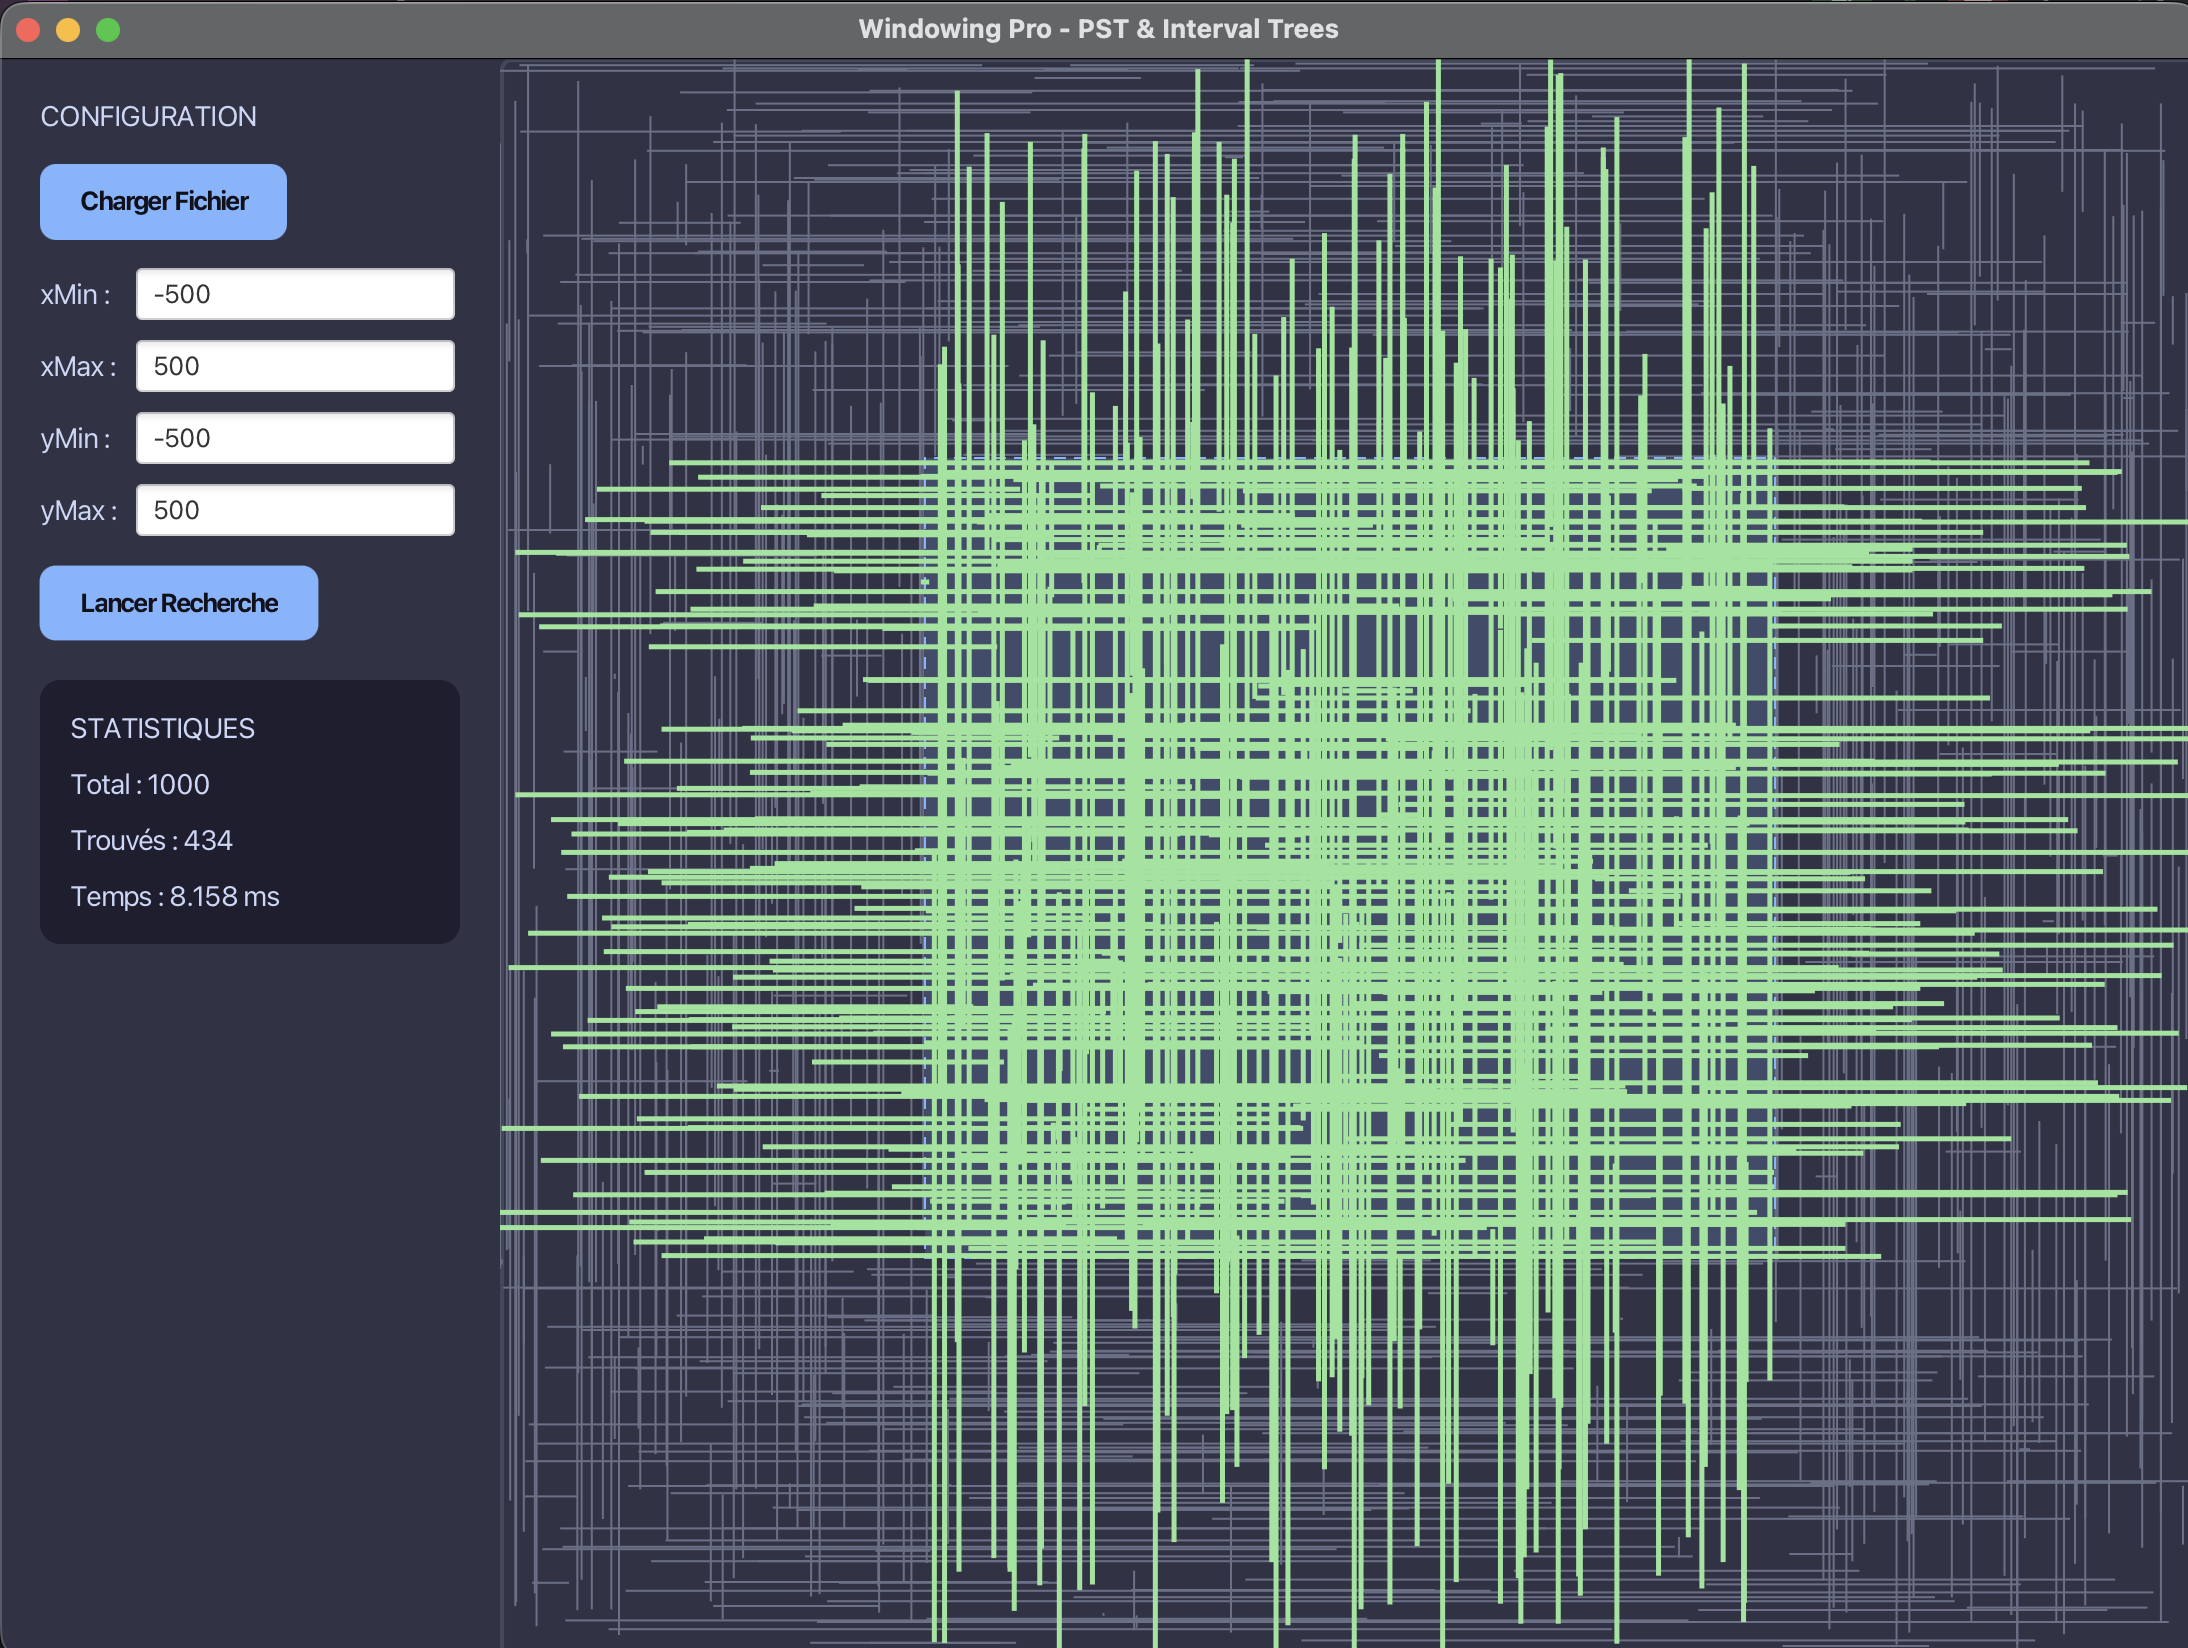
\includegraphics[width=0.85\textwidth]{screen_app1.png}
\caption{Interface après chargement d'un fichier de 1000 segments et lancement d'une recherche sur la fenêtre $[-500, 500] \times [-500, 500]$ : 434 segments trouvés en 8,158 ms. Les segments intersectant la fenêtre sont affichés en vert.}
\label{fig:gui1}
\end{figure}

\begin{figure}[h]
\centering
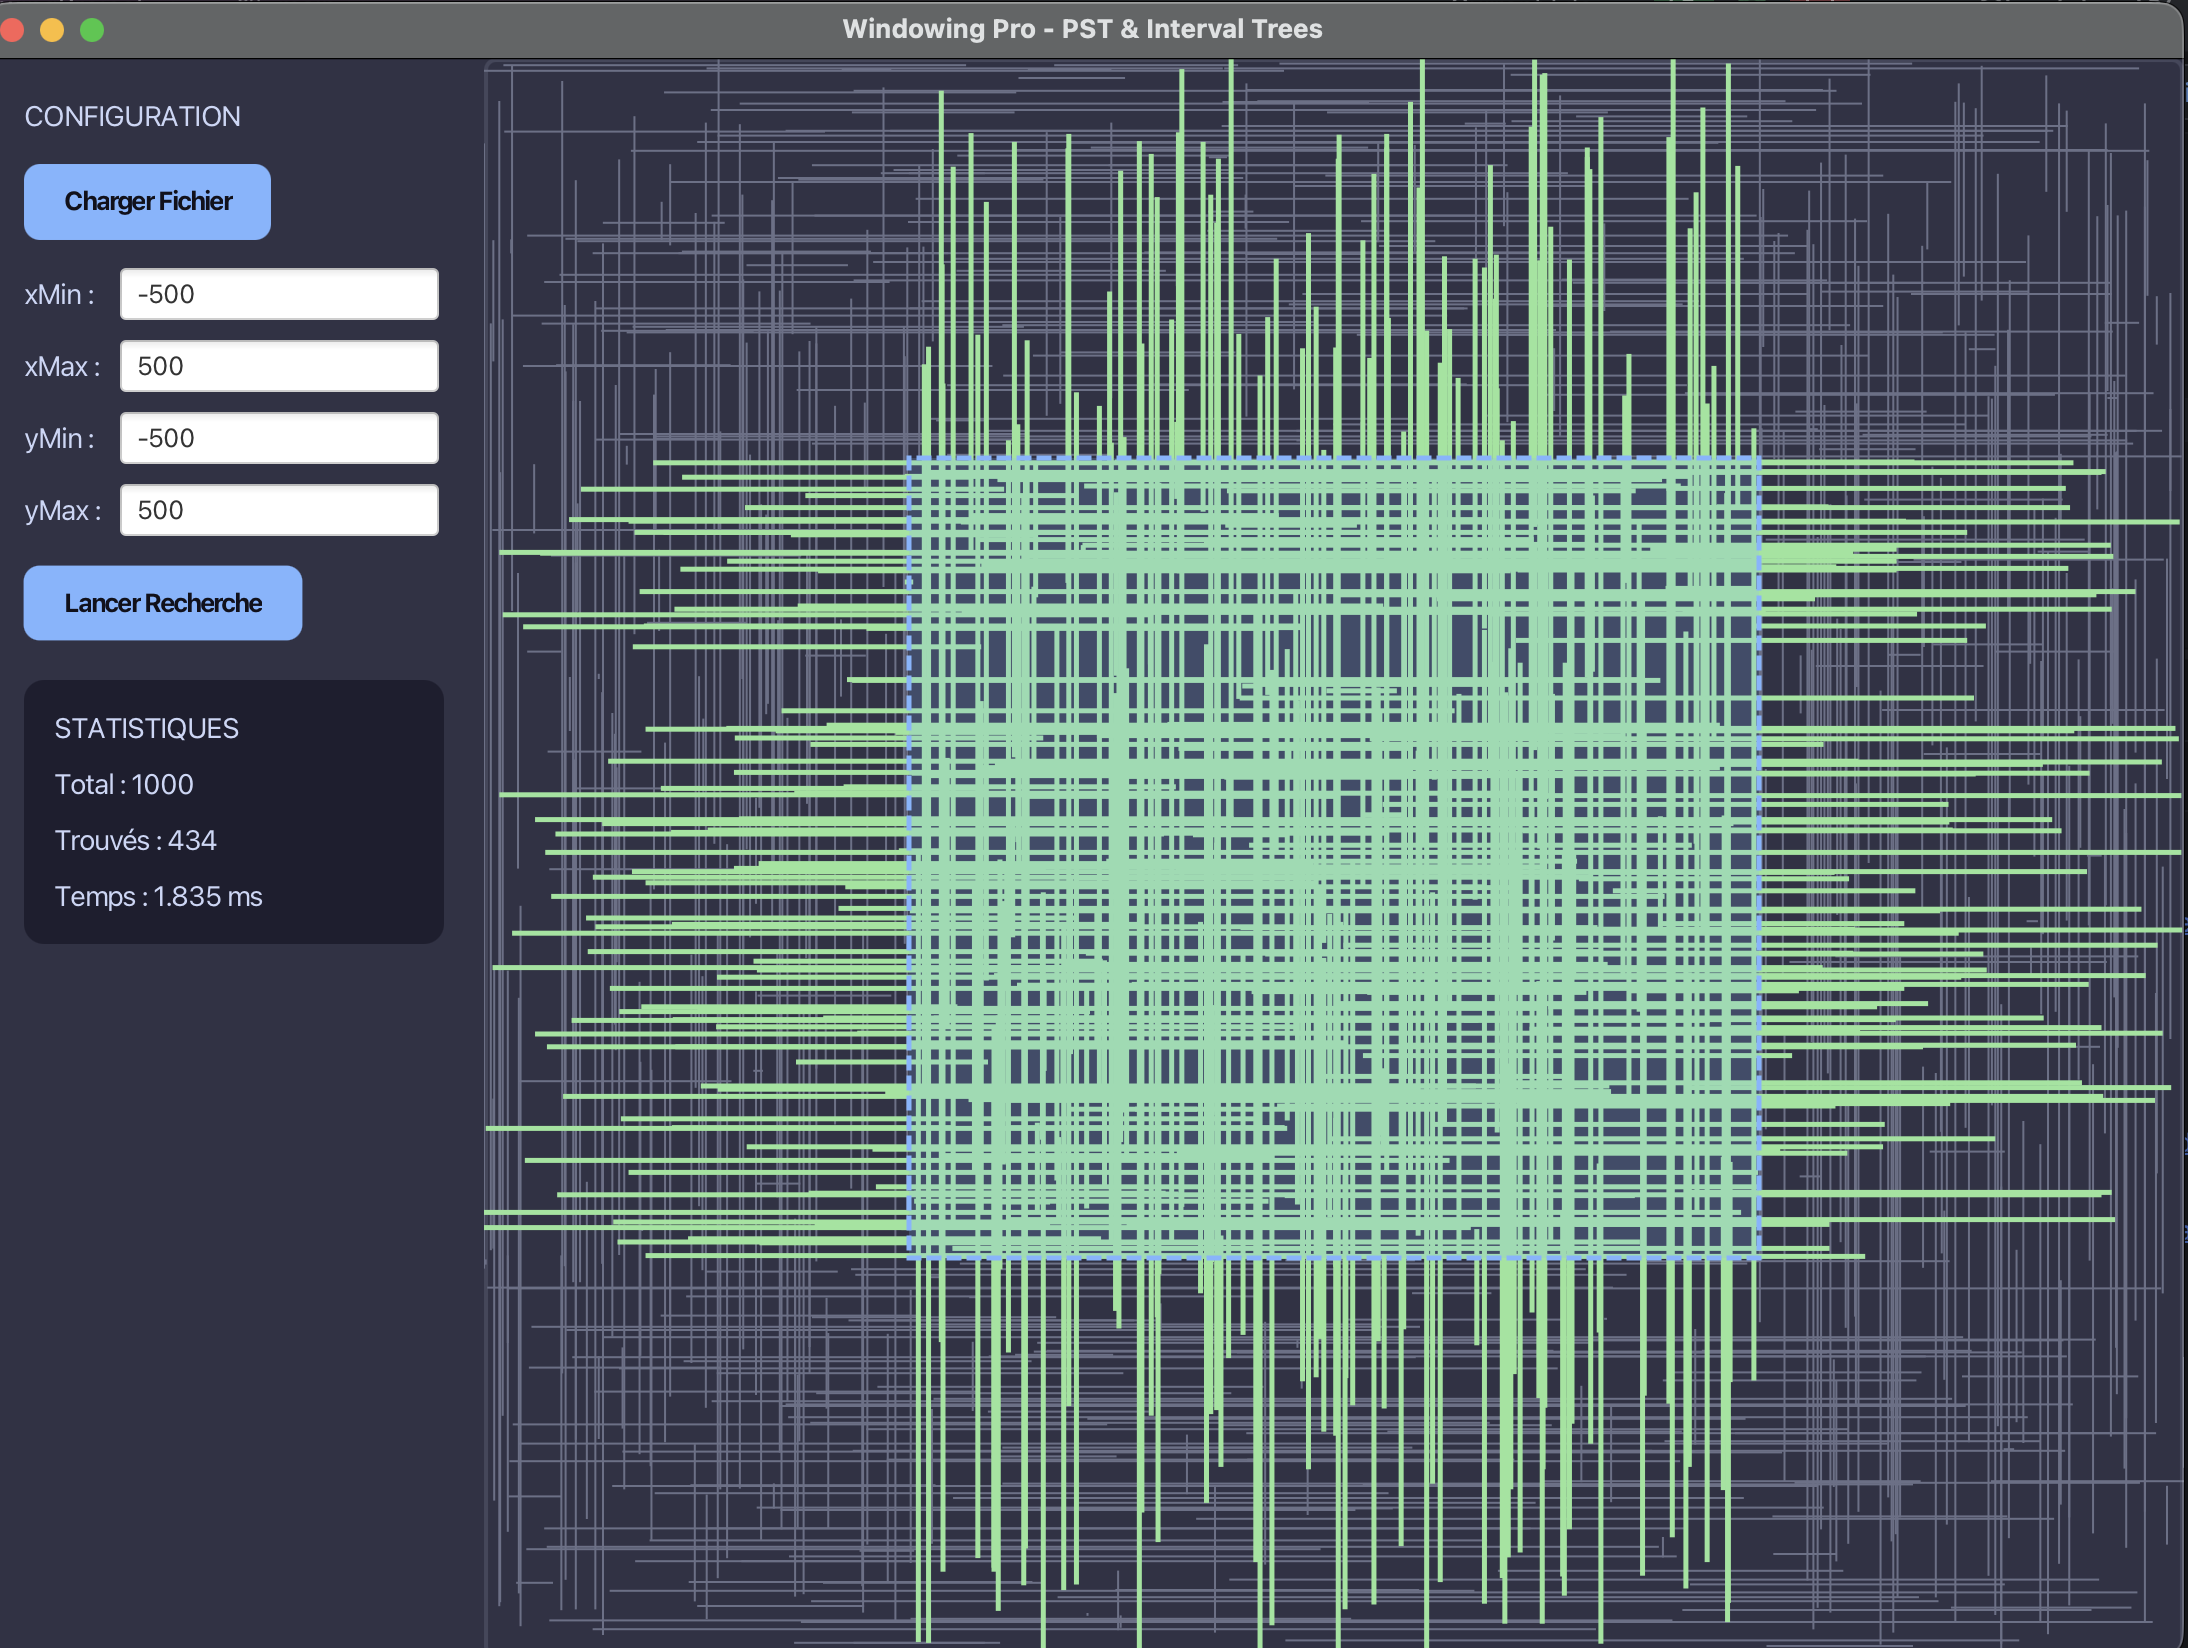
\includegraphics[width=0.85\textwidth]{screen_app2.png}
\caption{Résultat avec la fenêtre de requête (rectangle bleu pointillé) visible au premier plan. Les segments intersectant $W$ sont mis en évidence en vert, les autres en gris. Temps de requête : 1,835 ms.}
\label{fig:gui2}
\end{figure}

\subsection{Fonctionnalités}

\begin{enumerate}
    \item \textbf{Chargement de fichier} : le bouton « Charger Fichier » ouvre un sélecteur. Le fichier doit respecter le format : première ligne = fenêtre de visualisation \texttt{xMin xMax yMin yMax}, lignes suivantes = segments \texttt{x1 y1 x2 y2}.

    \item \textbf{Saisie manuelle des coordonnées} : les champs \texttt{xMin}, \texttt{xMax}, \texttt{yMin}, \texttt{yMax} acceptent des nombres décimaux ou les chaînes \texttt{-inf} / \texttt{+inf}. Un champ vide est interprété comme $-\infty$ ou $+\infty$ selon la borne.

    \item \textbf{Sélection par glisser-déposer} : l'utilisateur dessine directement la fenêtre de requête sur le canvas par un \textit{drag \& drop}. Les coordonnées écran sont converties en coordonnées monde selon la transformation :
    \[
        worldX = \frac{mouseX}{largeur} \times (x_{max} - x_{min}) + x_{min}
    \]

    \item \textbf{Affichage des résultats} : les segments intersectant $W$ apparaissent en vert, les autres en gris. La fenêtre est affichée en bleu pointillé au premier plan.

    \item \textbf{Statistiques} : le panneau indique le nombre total de segments, le nombre trouvés ($k$) et le temps d'exécution en millisecondes.
\end{enumerate}

% ==============================================================================
\section{Manuel de Compilation et d'Exécution}
% ==============================================================================

Le projet s'appuie sur \textbf{Maven} comme outil de gestion. Un wrapper \texttt{./mvnw} est fourni dans le répertoire racine.

\subsection{Prérequis}

\begin{itemize}
    \item Java 17 ou supérieur
    \item Maven (ou utiliser le wrapper \texttt{./mvnw})
\end{itemize}

\subsection{Commandes}

\begin{lstlisting}[language=bash, caption={Compilation et exécution}]
# Compilation
./mvnw compile

# Lancement de l'application
./mvnw javafx:run

# Exécution des tests
./mvnw test
\end{lstlisting}

\subsection{Format du fichier de données}

\begin{lstlisting}[caption={Exemple de fichier de données}]
-1000.0 1000.0 -1000.0 1000.0
652.0 -804.0 652.0 798.0
-49.0 211.0 -724.0 211.0
748.0 -636.0 777.0 -636.0
...
\end{lstlisting}

La première ligne définit la fenêtre de visualisation \texttt{[xMin xMax yMin yMax]}. Les lignes suivantes définissent les segments au format \texttt{x1 y1 x2 y2}.

% ==============================================================================
\section{Tests}
% ==============================================================================

Une suite de \textbf{60 tests unitaires} est fournie, organisée en cinq classes JUnit~5 :

\begin{table}[h]
\centering
\begin{tabular}{@{}llp{7cm}@{}}
\toprule
\textbf{Classe} & \textbf{Tests} & \textbf{Éléments testés} \\
\midrule
\texttt{CompositeNumberTest} & 11 & Ordre lexicographique, \texttt{lowerBound}, \texttt{upperBound}, \texttt{leq}, \texttt{geq}, cas aux bornes \\
\texttt{SegmentTest} & 14 & Intersection horiz./vert. avec diverses fenêtres, bornes infinies, contacts sur les bords \\
\texttt{PrioritySearchTreeTest} & 13 & \texttt{queryOpenLeft}, \texttt{queryYStrip}, PST négatif, coordonnées dupliquées, arbre vide \\
\texttt{IntervalTreeTest} & 12 & Croisement horiz./vert., arrêt précoce, cas aux limites, arbre vide/nul \\
\texttt{PstWindowingTest} & 10 & Algorithme complet : fenêtre bornée, semi-illimitée, déduplication \\
\midrule
\textbf{Total} & \textbf{60} & \textbf{Tous les modules couverts} \\
\bottomrule
\end{tabular}
\caption{Suite de tests unitaires — 60/60 tests passent avec succès.}
\end{table}

% ==============================================================================
\section{Conclusion}
% ==============================================================================

Ce projet met en œuvre une solution efficace au problème du fenêtrage pour des segments axis-parallèles, atteignant une complexité $\mathcal{O}(\log n + k)$ par requête grâce à la combinaison du PST et de l'Interval Tree. L'utilisation des nombres composites (Section 5.5 de Berg et al.) garantit la correction de l'algorithme même en présence de coordonnées dupliquées. Le patron Strategy offre une architecture extensible pour traiter toutes les configurations de fenêtre. L'interface JavaFX permet une visualisation interactive avec sélection de la fenêtre par glisser-déposer, et une suite de 60 tests unitaires valide l'ensemble des composants.

La transition d'une complexité linéaire $\mathcal{O}(n)$ vers une complexité optimale $\mathcal{O}(\log n + k)$ démontre l'impact critique du choix des structures de données pour des applications géométriques à grande échelle.

\end{document}
